\documentclass{article}
\usepackage{graphicx} % Required for inserting images
\usepackage[italian]{babel}
\usepackage[hidelinks]{hyperref}
\usepackage{todonotes}
\usepackage{biblatex}
\usepackage{listings}
\usepackage{parskip}
\usepackage{verbatim} 

\title{
    Project Management \\
    \textbf{ 
        Team Operating Rules \\ 
        for Web Application: \\
        \textit{Google CookBook}
    }
}
\author{
    Marica Pasquali \\ 
    (\href{mailto:marica.pasquali@studio.unibo.it}{marica.pasquali@studio.unibo.it})
}

\begin{document}

\maketitle 
\newpage
\tableofcontents 
\newpage

\section{Scrum Team e ruoli}

Il Scrum Team è composta dalle seguenti persone:

\begin{itemize}
    \item \textbf{Hannah}: Senior Full Stack Developer e Product Owner
    \item \textbf{Mirko}: Senior Full Stack Developer e Scrum Master
    \item \textbf{John}: Junior Front-End Developer
    \item \textbf{Kate}: Junior Front-End Developer
    \item \textbf{Carlo}: Junior Back-End Developer
    \item \textbf{Jane}: Junior Back-End Developer
    \item \textbf{Marco}: Database Administrator e Developer
\end{itemize}

\section{Team Values}

Lo Scrum Framework articola una serie di Valori Scrum per aiutare a guidare il lavoro, le azioni e il comportamento dei membri dello Scrum Team.

Gli Scrum Values sono:

\begin{figure}[h]
    \centering
    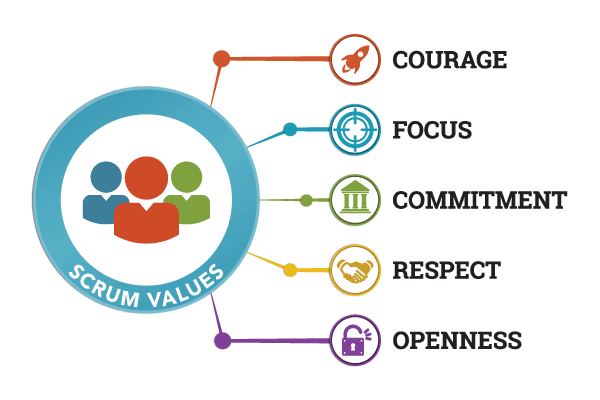
\includegraphics[scale=0.4]{./imgs/scrum-values.png}
\end{figure}

\begin{itemize}
    \item \textbf{Coraggio} - I membri dello Scrum Team hanno bisogno di coraggio per fare la cosa giusta e affrontare problemi difficili. 
    Ad esempio, dovrebbero mostrare il coraggio di esplorare l'ignoto, cambiare direzione, condividere informazioni e affrontare cortesi disaccordi.
    
    \item \textbf{Focus} - Lo Scrum Team si concentra sul lavoro dello Sprint e sui suoi obiettivi. 
    Esempi di ciò includono concentrarsi su: creazione di valore, ciò che è attualmente più importante e arrivare al Fatto.
    
    \item \textbf{Commitment} - Ciascun membro dello Scrum Team si impegna a raggiungere gli obiettivi del team e a sostenersi a vicenda. 
    Ciò comporta impegno o dedizione a:
    \begin{itemize}
        \item Fornire valore;
        \item Qualità;
        \item Lavorare verso gli obiettivi dello Sprint e del Prodotto;
        \item Usare l'empirismo.
    \end{itemize}

    
    \item \textbf{Rispetto} - E' necessario che i membri dello Scrum Team si rispettino a vicenda in quanto professionisti qualificati. 
    I membri dello Scrum Team dovrebbero rispettare le diverse competenze e prospettive degli altri ed essere rispettosi quando 
    non sono d'accordo.
     
    \item \textbf{Openness} - Lo Scrum Team e i suoi sponsors concordano di essere aperti riguardo a tutto il lavoro e alle sfide legate all'esecuzione del lavoro.
    I membri dello Scrum Team dovrebbero essere aperti riguardo alle difficoltà che devono affrontare. Dovrebbero condividere feedback e imparare gli uni 
    dagli altri e dalle parti interessate
\end{itemize}

\section{Problem solving}
Se si verifica un problema, i membri del team devono agire come segue:

\begin{figure}[h]
    \centering
    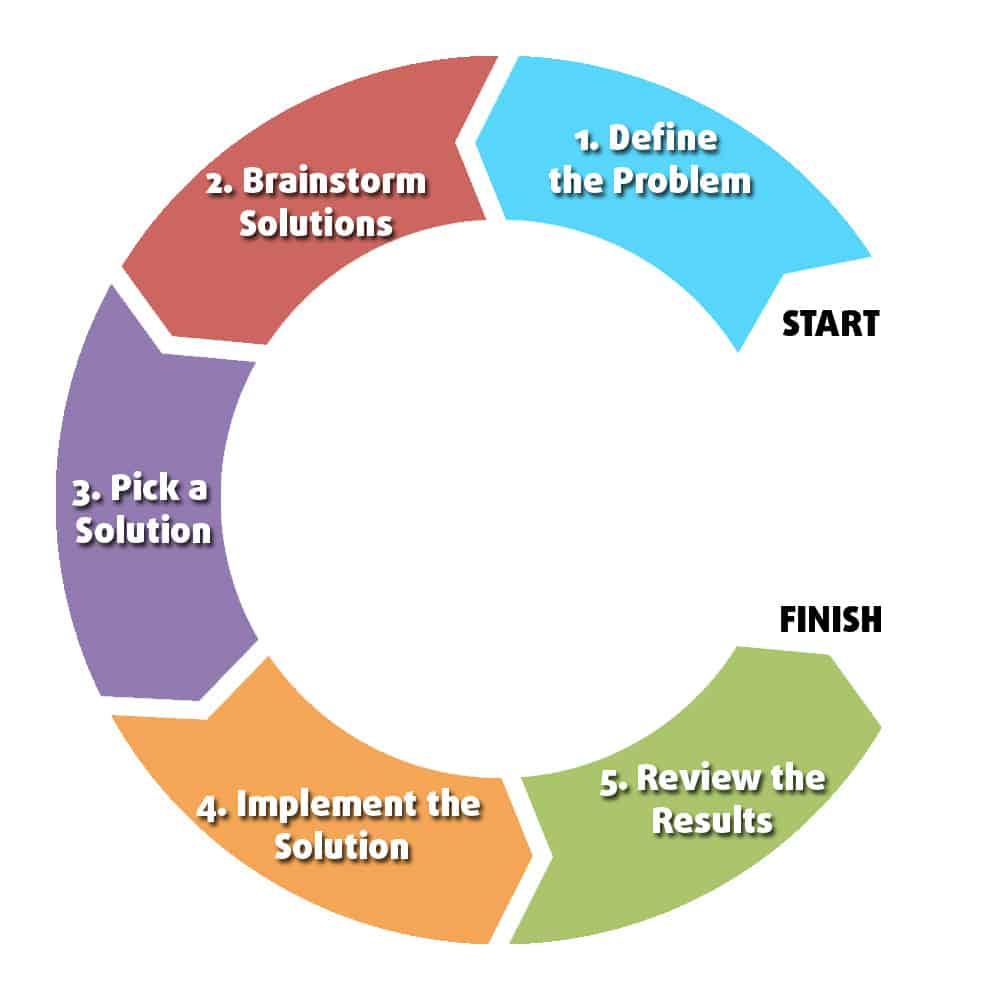
\includegraphics[scale=0.25]{./imgs/Problem-Solving-Cycle.jpg}
    \label{Problem Solving Cycle}
\end{figure}

\begin{enumerate}
    \item \textbf{Definire il problema}. Si esprima il problema in maniera più chiara possibile, identificado, se possibile, anche l'owner.
    L'owner portrebbe aiutare ad ottenere una descrizione più accurata del problema e quindi 
    anche le strategie per affrontalo.
    \item \textbf{Generare le possibili soluzioni}. Si elenchino tutte le possibili soluzioni, e si dia il via alla discussione.
    Si valutino in temini di vantaggi e svantaggi le soluzioni trovate. 
    \item \textbf{Scegliere una soluzione}. Si delinei la logistica dell'operazione dopo aver scelto la soluzione da implementare, ossia
    si specifichi chi interverrà, come la soluzione sarà implementata e quando la soluzione sarà implementata.
    \item \textbf{Implementare la soluzione scelta}. Si implementi la soluzione come pianificato
    \item \textbf{Valutare il risultato ottenuto}. Si valuti quanto la soluzione sia efficace e si decida se il piano esistente necessiti di essere rivisto, 
    o se un nuovo piano sia necessario per rispondere meglio al problema. 
    Se la soluzione non è soddisfacente, il processo può essere ripetuto.     
\end{enumerate}

\section{Decision making}
Per il processo di Decision Making si decide di seguire un approccio consultativo, in cui al
Product Owner o al Scrum Master spetta l'ultima parola (in base all'argomento trattato), 
ma solo dopo aver raccolto informazioni, idee e proposte dai membri del team. 
La sinergia tra i membri del team consente di individuare la migliore decisione e aumenta il 
loro coinvolgimento.

Nello specifico, il processo di Decision Making si distribuisce nei seguenti step:
\begin{enumerate}
    \item Viene discusso il tema su cui si è chiamati a prendere una decisione,
    allo scopo di individuare pareri e informazioni.
    \item Viene formulata una proposta.
    \item Ogni membro del gruppo attivamente mostra il suo accordo con la proposta.
    \item Se non si raggiunge il consenso, ciascun dissenziente presenta 
    la propria obiezione, che può far partire un altro ciclo di discussione per affrontare
    e chiarire l'obiezione.
    \item La proposta viene riformulata, nel tentativo di affrontare le obiezioni dei decisori. 
    Si ripete poi la verifica del consenso fino a quando una decisione soddisfacente non viene presa.
\end{enumerate}

\section{Team meetings}

Come già spiegano nel documento \textit{Planning Approch} (redatto nella fase di Planning), i vari meeting sono suddivisi in:
\begin{enumerate}
    \item \textbf{Sprint Planning}: riunione condotta prima di iniziare uno Sprint per un massimo di 4 ore.
    Durante questa riunione si pianifica il lavoro da svolgere nello Sprint attuale e si 
    prepara lo Sprint Backlog che dettagli il tempo necessario per fare quel lavoro. 
    Il piano è creato dal lavoro collaborativo dell'intero Team Scrum (Product Owner, Scrum Master, e team di sviluppo).
    Possono partecipare anche tutti i manager del caso interessati o i rappresentanti della clientela.

    \item \textbf{Daily Scrum}: riunione condotta ogni giorno ad inizio mattinata per massimo di 15 minuti. 
    Durante questa riunione ogni membro del team discute brevemente il lavoro svolto il giorno prima, 
    quello che prevede di svolgere il giorno corrente e se è presente qualche difficoltà nel raggiungere 
    gli obiettivi
    
    \item \textbf{Sprint Review}: riunione condotta dopo ogni Sprint (di durata 2 settimane) per un massimo di 2 ore.
    Durante questa riunione vengono discussi i risultati dello sprint precedente
    e vengono pianificate le attività da svolgere durante lo sprint corrente
    
    \item \textbf{Sprint Retrospective}: riunione condotta dopo la Sprint Review e
    prima del successivo Sprint Planning per un massimo di 1 ora e mezza. 
    Durante questa riunione viene discusso se c'è il bisogno di un piano di miglioramento 
    da attuare durante il prossimo Sprint.
\end{enumerate}

Nel caso durante lo svolgimento del progetto si è riscontrato un particolare problema si può organizzare una riunioni straordinaria
(\textbf{Problem resolution meeting}), in cui partecipano solo i membri che sono coinvolti direttamente nel problema. 
Solo in casi estremi, in cui non si riesce in nessun modo a trovare una soluzione potranno essere convocati anche gli altri membri.

\section{Piano di qualità tecnica}

Si è deciso di adottare le seguenti Good Practices per raggiungere l'obiettivo dell'eccellenza tecnica.

\begin{itemize}
  \item Utilizzo di un repository per ogni sottoprogetto
  \item Utilizzo di \href{https://www.atlassian.com/it/git/tutorials/comparing-workflows/gitflow-workflow}{GitFlow} all'interno di ogni repository
  \item Utilizzo di \href{https://www.conventionalcommits.org/en/v1.0.0/}{Conventional Commits} per la scrittura dei commit
  \item Commit scritti rigorosamente in inglese
  \item Utilizzo di un sistema di \href{https://en.wikipedia.org/wiki/CI/CD}{CI/CD} per l'automazione dei test e del deploy
  \item Utilizzo di un build tool per la risoluzione delle dipendenze date da librerie esterne
  \item Utilizzo di sistema automatico per la gestione dell'update delle versioni delle librerie esterne
  \item Inclusione della documentazione in ogni repository
  \item Scrittura di commenti all'interno del codice seguendo le convenzioni del linguaggio
  \item Utilizzo di pattern di programmazione consolidati per garantire riusabilità, scalabilità ed estensibilità del codice
  \item Controllo automatico della compatibilità di tutte le licenze utilizzate
  \item Conteinerizzazione del codice
  \item Adozione di un \href{https://en.wikipedia.org/wiki/Lint_(software)}{linter} automatico per la formattazione del codice seguendo le convenzioni del linguaggio
  \item Utilizzo di un tool per l'identificazione di codice ripetuto all'interno dello stesso progetto
\end{itemize}


\end{document}